\chapter{Application For Vehicle Couting Based On Density Estimation}

In this thesis, the application will develop to serve the client to count different types of vehicle or the different type of objects. So that, the application will support user create object types, get samples from a video then help client making training data from that samples. Assisting client for training and estimate the number of objects.
From that application has features:
\begin{enumerate}
  \item Get sample from video, and mark object with height and width.
  \item Train model with sample create from the first feature.
  \item Run the estimation with model train from the second feature.
\end{enumerate}
Application has been divide into  3 main module
\begin{enumerate}
  \item Marker: for get sample from video, define object types, mark object of object types in samples.
  \item Trainer: Train model with sample create from Marker.
  \item Runner: Run the estimation with model train from Trainer.
\end{enumerate}
\section{Use Case Description}
\begin{center}
  \begin{figure}[H]
    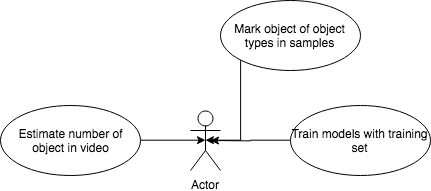
\includegraphics[width=\textwidth]{Chapters/Fig/usecase}
    \label{usecasediagram}
    \caption{Use Case Diagram}
  \end{figure}
\end{center}

\begin{table}[H]
\begin{center}
  \begin{tabular}{ | c | l | } 
  \hline
  \textbf{Actor} & \textbf{Use case} \\
  \hline
  \multirow{3}{4em}{Client} & Mark object of object types in samples. \\
  &Train models with training set. \\
  &Estimate number of object in video. \\
  \hline
  \end{tabular}
  
\end{center}
\caption{Use Case Table}\label{tab:usecase}
\end{table}

\begin{table}[H]
  \begin{center}
    \begin{tabular}{ | c | l | } 
    \hline
    \textbf{Use case ID} & UC01 \\
    \hline
    \textbf{Use case name} & Mark object of object types in samples \\
    \hline
    \textbf{Description} & Mark object of object types in samples\\
    \hline
    \textbf{Actor} & Client \\
    \hline
    \textbf{Trigger} & Open marker tab \\
    \hline
    \textbf{Input} & Object type, samples \\
    \hline
    \textbf{Output} & Show mark in viewer and extract to training set \\
    \hline    
    \multirow{2}{4em}{\textbf{Preconditions}} & 1. Open the application, click on Marker button. \\ 
    & 2. Objects has been added, get sample from video, lock the object types. \\
    \hline
    \multirow{16}{4em}{\textbf{Main Flow}}  & 1. Select sample on list of samples.\\
    & 2. Click object type on list of object types. \\
    & 3. Click "Add Object" button. \\ 
    & 4. Set height (click 3 point in viewer), width (click 1 point in viewer). \\
    & 5. Click "Done" button (The viewer will update mark when \\
    & click "Done" button). \\
    & 6. If the mark is not satisfies the client desire, \\
    & click "Clear" button and go back step 3. \\
    & 7. Go back step 3 until all object of that object types is marked. \\
    & 8. Go back step 2 until all object types on that sample is marked. \\
    & 9. Go back step 1 until the client do not need more images for traning set \\
    & or out of sample on the list samples. \\
    & 10. If Client need more samples add to list of samples \\
    & then select number of sample need on the left of "Add more samples" button \\
    & and click "Add more samples" button and go back step 1. \\
    & 11. Click "save obj to disk" button select the folder to save training set\\
    & list of oject types.\\
    \hline
    \textbf{Alternative Flow} & None \\
    \hline
    \textbf{Exceptions} & None \\
    \hline
    \textbf{Frequency of use} & Normal \\
    \hline
    \end{tabular}
  \end{center}
  \caption{Use Case UC01}\label{tab:uc1}
\end{table}

\begin{table}[H]
  \begin{center}
    \begin{tabular}{ | l | l | } 
    \hline
    \textbf{Use case ID} & UC02 \\
    \hline
    \textbf{Use case name} & Train models with training set. \\
    \hline
    \textbf{Description} & Train models with training set.\\
    \hline
    \textbf{Actor} & Client \\
    \hline
    \textbf{Trigger} & Click train button. \\
    \hline
    \textbf{Input} & Number of iter, same size gauss \\
    \hline
    \textbf{Output} & Show status: "Train done" \\
    \hline    
    \textbf{Preconditions} & Has training set from marker, open the application \\
    \hline
    \multirow{6}{4em}{\textbf{Main Flow}}  & 1. Click "Train" button, train dialog will shows \\
    & 2. Click "Open Folder" button, choose folder that marker data saved \\
    & 3. Click "Open Dictionary File" button, choose dictionary file in csv form. \\
    & 4. If client want all object of that object types has save size then \\
    & click "Kernel gauss's size same for all object" check button  \\
    & 5. Click "Start Train" button. \\
    \hline
    \textbf{Alternative Flow} & None \\
    \hline
    \textbf{Exceptions} & None \\
    \hline
    \textbf{Frequency of use} & Normal \\
    \hline
    \end{tabular}
  \end{center}
  \caption{Use Case UC02}\label{tab:uc2}
\end{table}


\begin{table}[H]
  \begin{center}
    \begin{tabular}{ | l | l |} 
    \hline
    \textbf{Use case ID} & UC03 \\
    \hline
    \textbf{Use case name} & Estimate number of object in video. \\
    \hline
    \textbf{Description} & Estimate number of object in video. \\
    \hline
    \textbf{Actor} & Client \\
    \hline
    \textbf{Trigger} & Click "Run" button.\\
    \hline
    \textbf{Input} & Average all object types height, width; downscale; frame step  \\
    \hline
    \textbf{Output} & Show estimate data, and frame process \\
    \hline    
    \textbf{Preconditions} & Has data from marker, trainer, Open the application \\
    \hline
    \multirow{12}{4em}{\textbf{Main Flow}} &   1. Click "Run" button. \\
    & 2. Click "Open Video File" button then choose video file. \\
    & 3. Click "Open Folder" button then choose the folder \\
    & that contains data from marker \& trainer. \\
    & 4. Click "Open Dictionary File" button choose dictionary file in .csv form. \\
    & 5. Client need to change average object types size (height, width). \\
    & 6. If client want downscale sample, click "Downscale Sample" check button \\
    & set downscale sample scale if want to change value (default value is 0.5). \\
    & 7. If client want to change frame set \\
    & (which is number of frame between 2 continuous samples) \\
    & then change the value of framestep (default value is 5). \\
    & 8. Click $>$ button to start run estimate. \\
    \hline
    \textbf{Alternative Flow} & None \\
    \hline
    \textbf{Exceptions} & None \\
    \hline
    \textbf{Frequency of use} & Normal \\
    \hline
    \end{tabular}
  \end{center}
  \caption{Use Case UC03}\label{tab:uc3}
\end{table}
\pagebreak
\section{Algorithms}
\subsection{Training}
 \textbf{FOR ALL} object types as \textbf{objectType} in list of object types \textbf{DO}
        \begin{enumerate}
          \item  Calculate Dense-SIFT of each sample of \textbf{objectType} 
          \item  Calculate features of each sample of \textbf{objectType} 
          \item  Calculate ground truth of each sample of \textbf{objectType} 
          \item  Train model for that \textbf{objectType} 
        \end{enumerate}
 \subsection{Estimation}
        \begin{enumerate}
          \item  Calculate Dense-SIFT of each sample of \textbf{objectType} 
          \item  Calculate features of each sample of \textbf{objectType} 
          \item  Load model of \textbf{objectType} 
          \item  Estimation with model loaded from previous step for \textbf{objectType} 
        \end{enumerate}

\section{Implementation}
This chapter presents environment configurations and details of implementations of application. \\
\subsection{Environment Configurations}
\begin{table}[H]
  \begin{center}
    \begin{tabular}{ | l | l |} 
    \hline
    \textbf{OS} & Mac OS  10.11.6 \& 10.13.4\\
    \hline
    \textbf{CPU} & i7-3770K @ 3.50GHz \& i7-7820HQ @ 2.9Ghz \\
    \hline
    \textbf{RAM} & 16GB 1600 Mhz DDR3 \& 16GB 2133 Mhz LPDDR3 \\
    \hline
    \textbf{CMAKE} & 3.10.0 \\
    \hline
    \textbf{QT} & Qt: stable version 5.10.1 \\
    \hline
    \textbf{Qpencv} & Stable version 3.4.1 \\
    \hline
    \textbf{cvxopt} & Version 1.1.9 \\
    \hline
    \textbf{vlfeat} & Version 0.9.20 \\
    \hline
    \end{tabular}
  \end{center}
  \caption{Environment Configurations}\label{tab:Environmentconfigurations}
\end{table}


\subsection{Main classes}

The application is implemented in $C++$ language and QT framework with following module:\\
\textbf{Marker: }
\begin{itemize}
  \item \textbf{dialogmarker.ui} File that contains config for UI for dialog marker
  \item \textbf{dialogmarker.cpp} $C++$ source code that handle the UI signal and connect UI with \textbf{MarkingWorker}
  \item \textbf{dialogmarker.h} Header of Dialog that define UI
  \item \textbf{MarkingWorker.cpp} $C++$ source code of worker that use in UI for doing Job for UI, handle marking data
  \item \textbf{MarkingWorker.h} Header of worker that use in UI for doing Job for UI
\end{itemize}

\textbf{Trainer: }
\begin{itemize}
  \item \textbf{dialogtrain.ui} File that contains config for UI for dialog train
  \item \textbf{dialogtrain.cpp} $C++$ source code that handle the UI signal and connect UI with \textbf{TrainingWorker}
  \item \textbf{dialogtrain.h} Header of Dialog that define UI
  \item \textbf{TrainingWorker.cpp} $C++$ source code of worker that use in UI for doing Job for UI, \textbf{where learning method integrated}
  \item \textbf{TrainingWorker.h} Header of worker that use in UI for doing Job for UI
  \item \textbf{ListModel.cpp} $C++$ source code of samples and object types models for table show in list view 
  \item \textbf{ListModel.h} Header of \textbf{ListModel.cpp}
\end{itemize}

\textbf{Runner: }
\begin{itemize}
  \item \textbf{dialogrun.ui} File that contains config for UI for dialog run
  \item \textbf{dialogrun.cpp} $C++$ source code that handle the UI signal and connect UI with \textbf{MarkingWorker}
  \item \textbf{dialogrun.h} Header of Dialog that define UI
  \item \textbf{RunningWorker.cpp} $C++$ source code of worker that use in UI for doing Job for UI, \textbf{handle estimate of counting objects in video}
  \item \textbf{RunningWorker.h} Header of worker that use in UI for doing Job for UI
  \item \textbf{SampleDetail.cpp} $C++$ source code of Model data for table show in list view 
  \item \textbf{SampleDetail.h} Header of \textbf{SampleDetail.cpp}
\end{itemize}

\textbf{Not in Any module: }
\begin{itemize}
  \item \textbf{ObjectMark.cpp} $C++$ source code for store marker data 
  \item \textbf{ObjectMark.h} Header of \textbf{ObjectMark.cpp}
  \item \textbf{ViewerLabel.cpp} $C++$ source code For make label become viewer and clickable 
  \item \textbf{ViewerLabel.h} Header file of \textbf{ViewerLabel.cpp}
\end{itemize}

The following diagrams is class diagram of main class:

\begin{center}
  \begin{figure}[H]
    \centering
    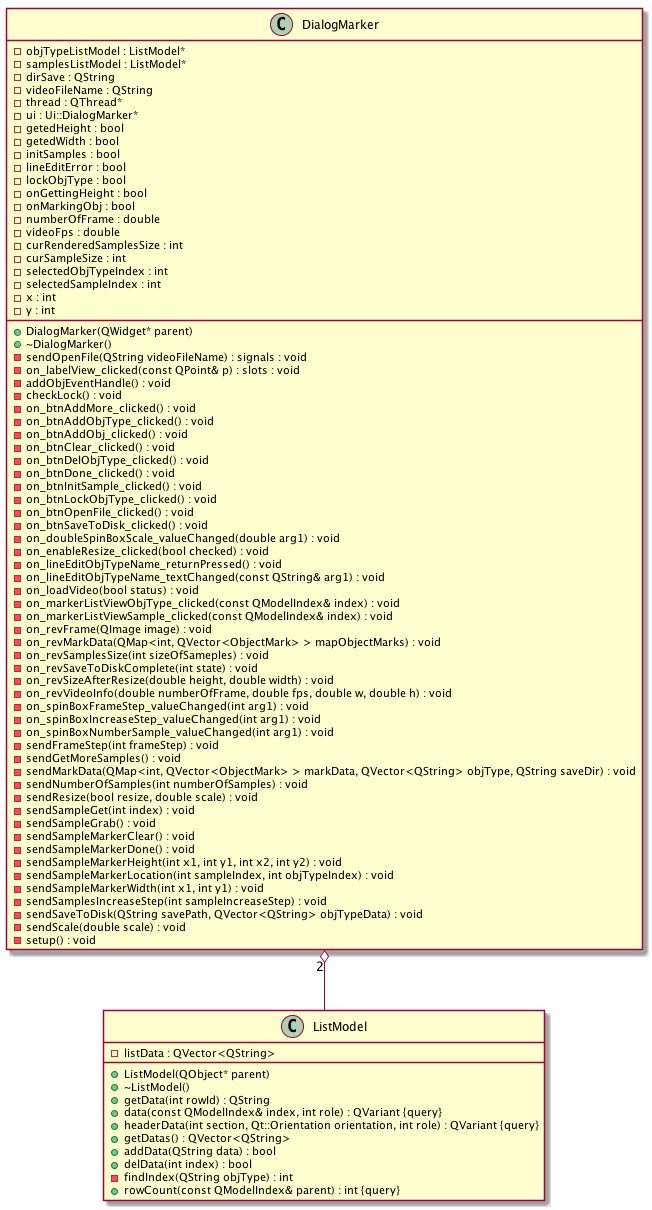
\includegraphics[height=0.9\textheight]{Chapters/Fig/dmarkerd}
    \caption{Class Diagram}
    \label{fig:cd-marker}
  \end{figure}
  \begin{figure}[H]
    \centering
    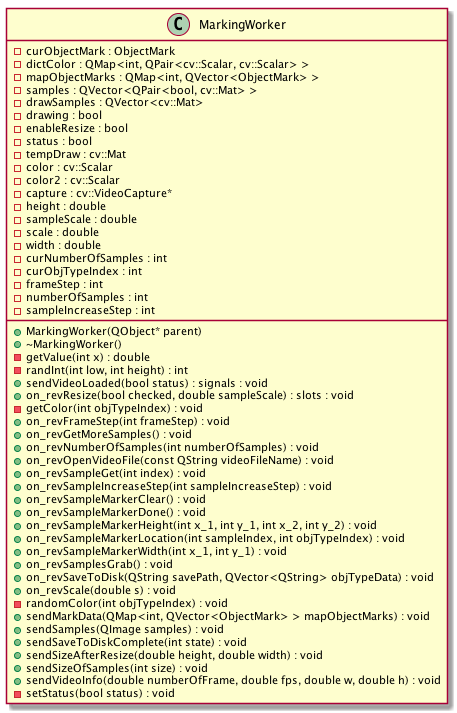
\includegraphics[height=0.8\textheight]{Chapters/Fig/wmarkerd}
    \caption{Class Diagram}
    \label{fig:cd-mworker}
  \end{figure}
  \begin{figure}[H]
    \centering
    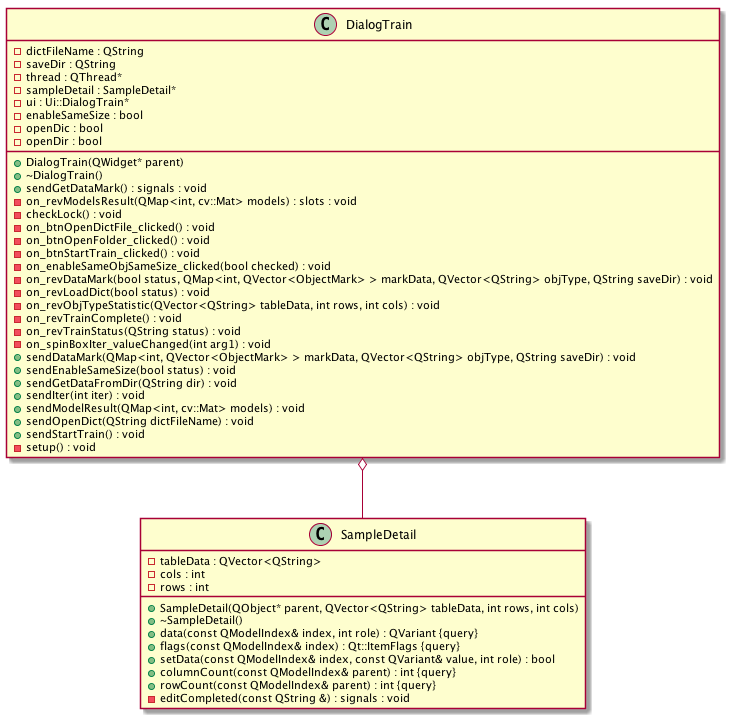
\includegraphics[height=0.65\textheight]{Chapters/Fig/dtraind}
    \caption{Class Diagram}
    \label{fig:cd-train}
  \end{figure}
  \begin{figure}[H]
    \centering
    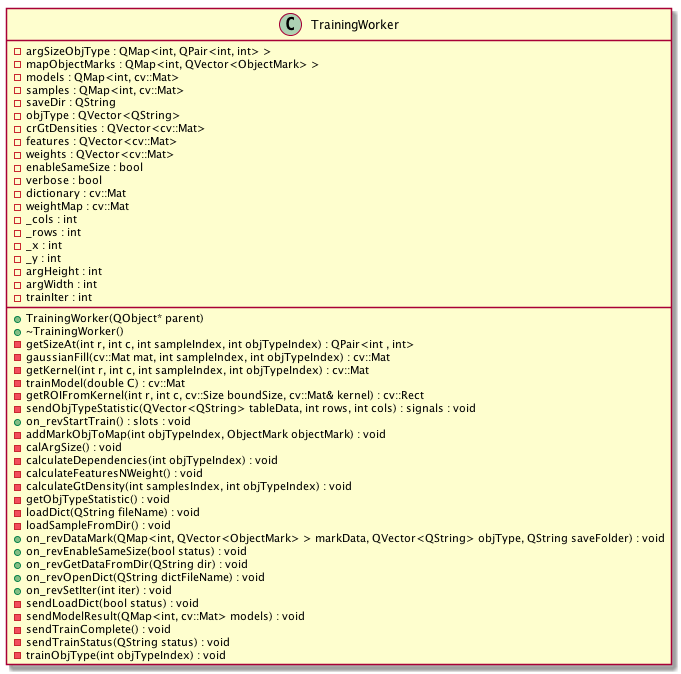
\includegraphics[height=0.68\textheight]{Chapters/Fig/wtraind}
    \caption{Class Diagram}
    \label{fig:cd-tworker}
  \end{figure}
  \begin{figure}[H]
    \centering
    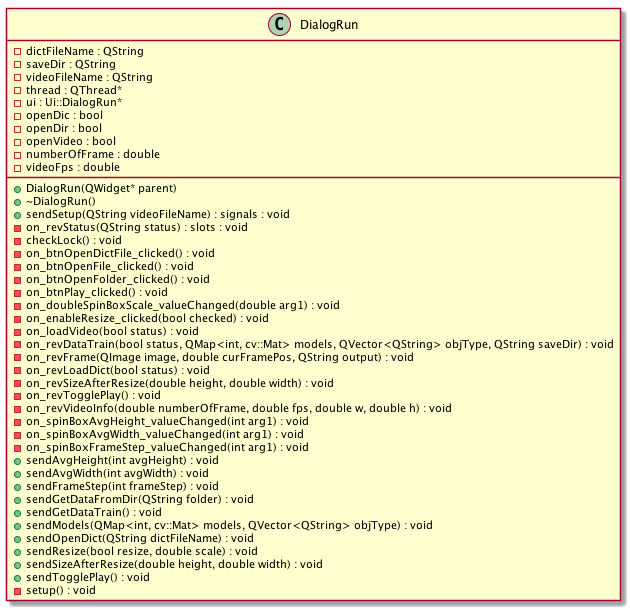
\includegraphics[height=0.6\textheight]{Chapters/Fig/drund}
    \caption{Class Diagram}
    \label{fig:cd-run}
  \end{figure}
  \begin{figure}[H]
    \centering
    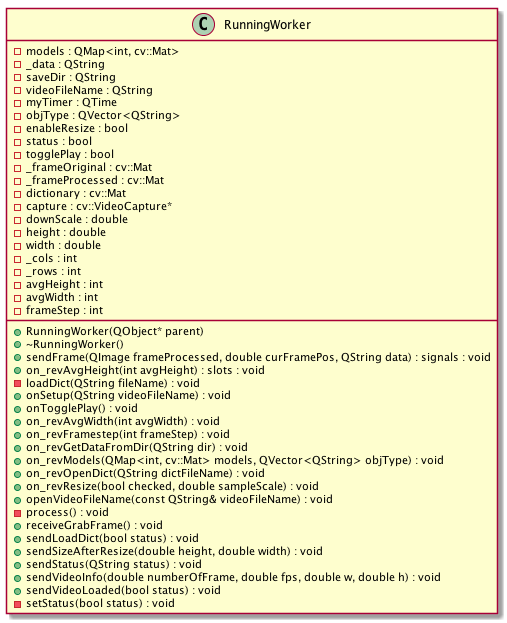
\includegraphics[height=0.65\textheight]{Chapters/Fig/wrund}
    \caption{Class Diagram}
    \label{fig:cd-rworker}
  \end{figure}
\end{center}

\subsection{Main Features}

\begin{center}
  \begin{figure}[H]
      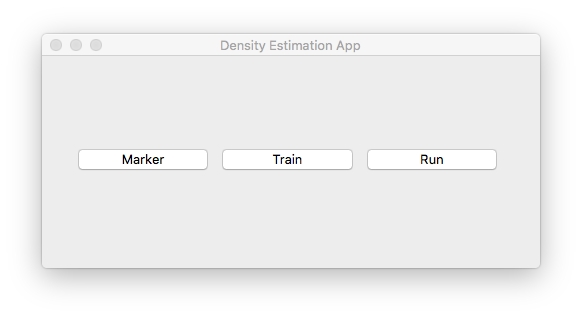
\includegraphics[width=\textwidth]{Chapters/Fig/Appllication}
      \caption{The Main Application}
      \label{fig:mainapp}
    \end{figure}
  \end{center}
  \begin{center}
\end{center}

Main application on figure \ref{fig:mainapp} where show 3 features to choose Marker, Train, Run

\begin{center}
    \begin{figure}[H]
      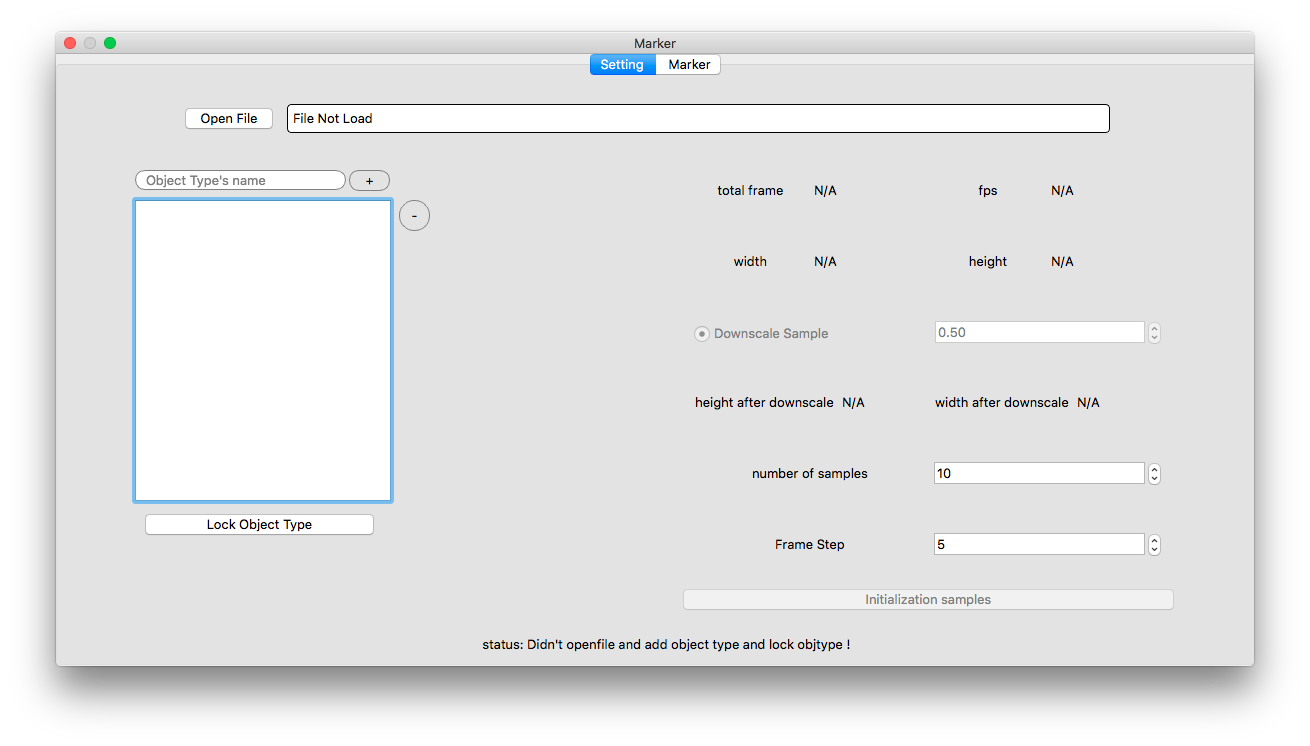
\includegraphics[width=\textwidth]{Chapters/Fig/marker-setting}
      \caption{The Setting Tab in Marker Dialog}
      \label{fig:marker-setting}
    \end{figure}
  \end{center}
  \begin{center}
\end{center}

In setting tab on figure \ref{fig:marker-setting} client config the setting of marker. 
\textbf{Downscale sample} where set the scale value for downscale in order to improve speed of training pharse.
\textbf{Number of sample} Where setting initialization of sample to mark.
\textbf{Frame step} Where setting frame between 2 continuous samples get in video.

\begin{center}
  \begin{figure}[H]
    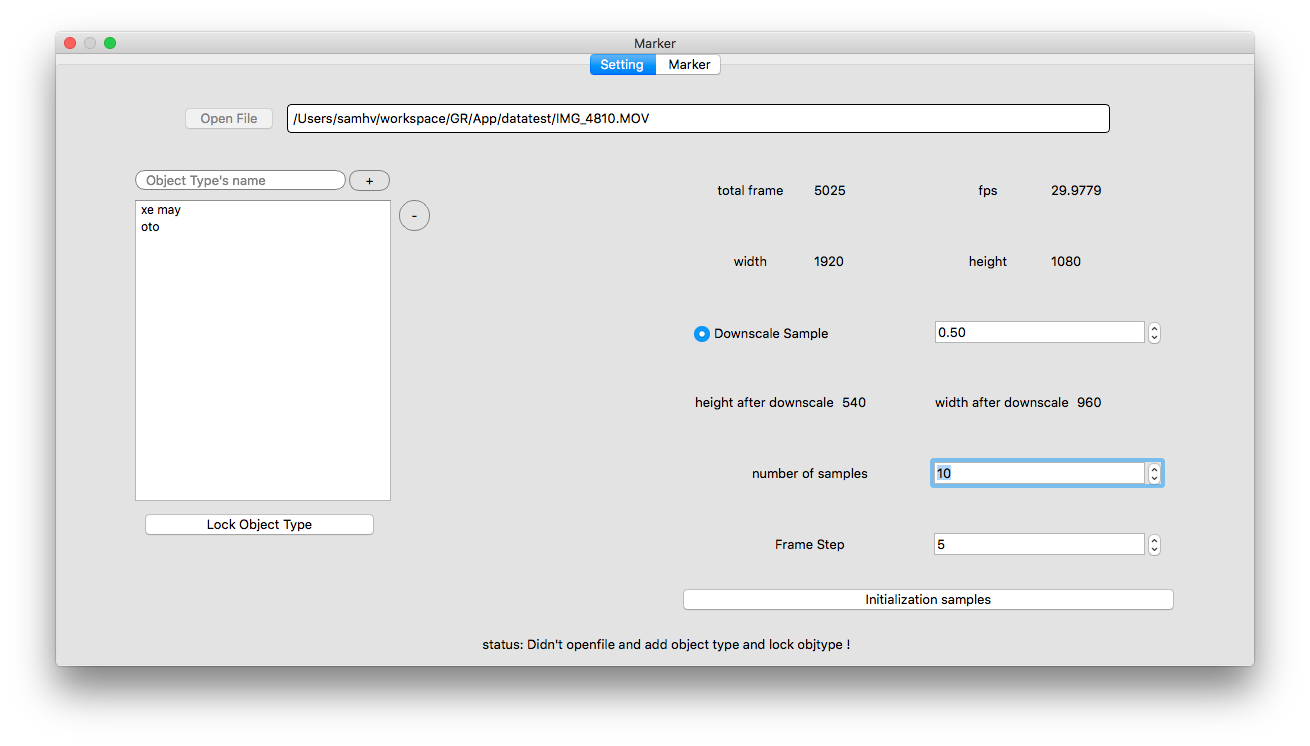
\includegraphics[width=\textwidth]{Chapters/Fig/setting-marker}
    \caption{Example of Setting Tab in Marker Dialog}
    \label{fig:Setting-marker}
  \end{figure}
\end{center}
\begin{center}
\end{center}

\begin{center}
    \begin{figure}[H]
      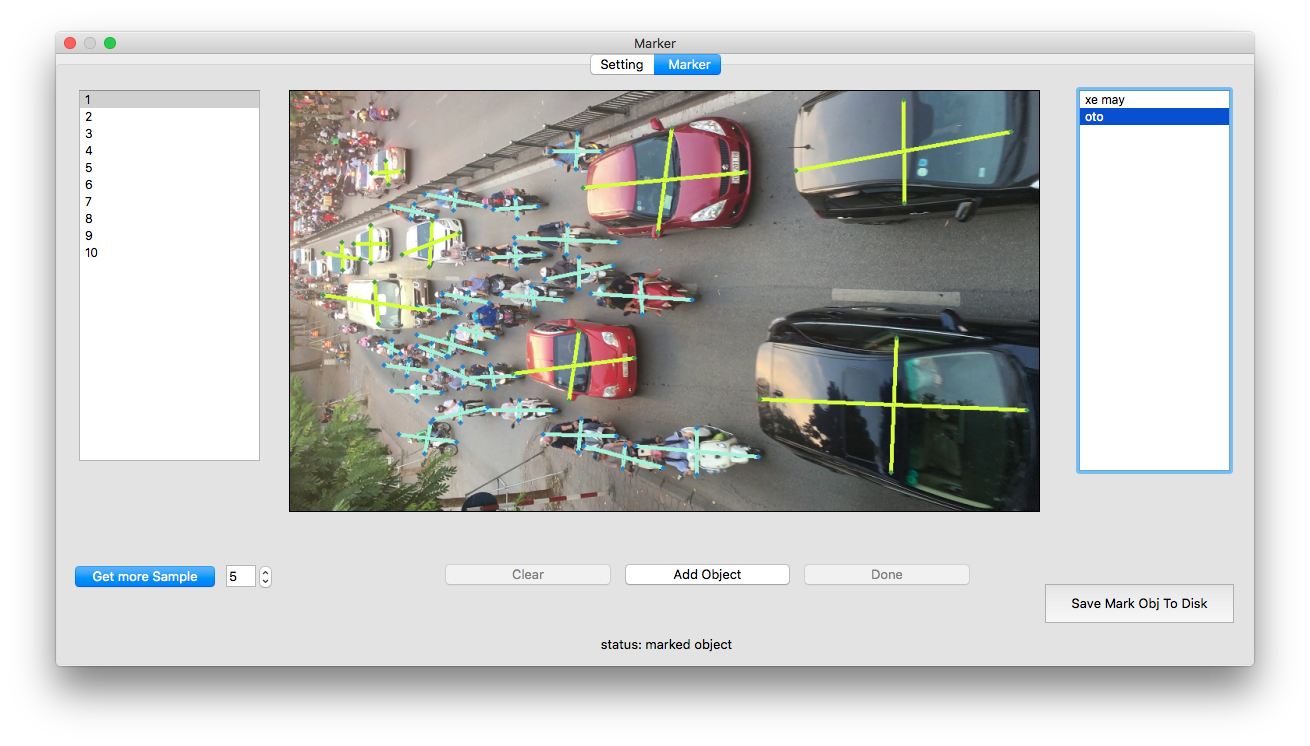
\includegraphics[width=\textwidth]{Chapters/Fig/marker-set}
      \caption{Marker Tab in Marker Dialog}
      \label{fig:marker-set}
    \end{figure}
  \end{center}
  \begin{center}
\end{center}

In figure \ref{fig:marker-set} shows the screen of the marker after mark the object in sample 1. On the left list show the list of samples that we get when clicking on "initialization samples" button on setting tab. On the right list shows the list of object types has been added in setting tab. The get more button help client can get more sample if the client need for more training images for the training set, the number of samples to get can config by change the number on the left of the button (default value is 5 sample). 

\begin{center}
    \begin{figure}[H]
      \includegraphics[width=\textwidth]{Chapters/Fig/trainer}
      \caption{The Trainer Dialog}
      \label{fig:Trainer}
    \end{figure}
  \end{center}
  \begin{center}
\end{center}

Fig \ref{fig:Trainer} shows the trainer dialog on training models for object types. The client must load the samples and dictionary for the train the model by click Open folder and Open Dictionary File buttons. If the client didn't close application after creating the dataset from marker dialog the information of saving data folder will auto load. The list of object type will load an show in the table with the number of the object has been marked. The Kernel Gauss's size same for all object check button if check will make all object with the same size with value of average size in that object type. The number of iterations of learning function can be set when to change the value of \textbf{Number of iterations}. \\

\begin{center}
    \begin{figure}[H]
      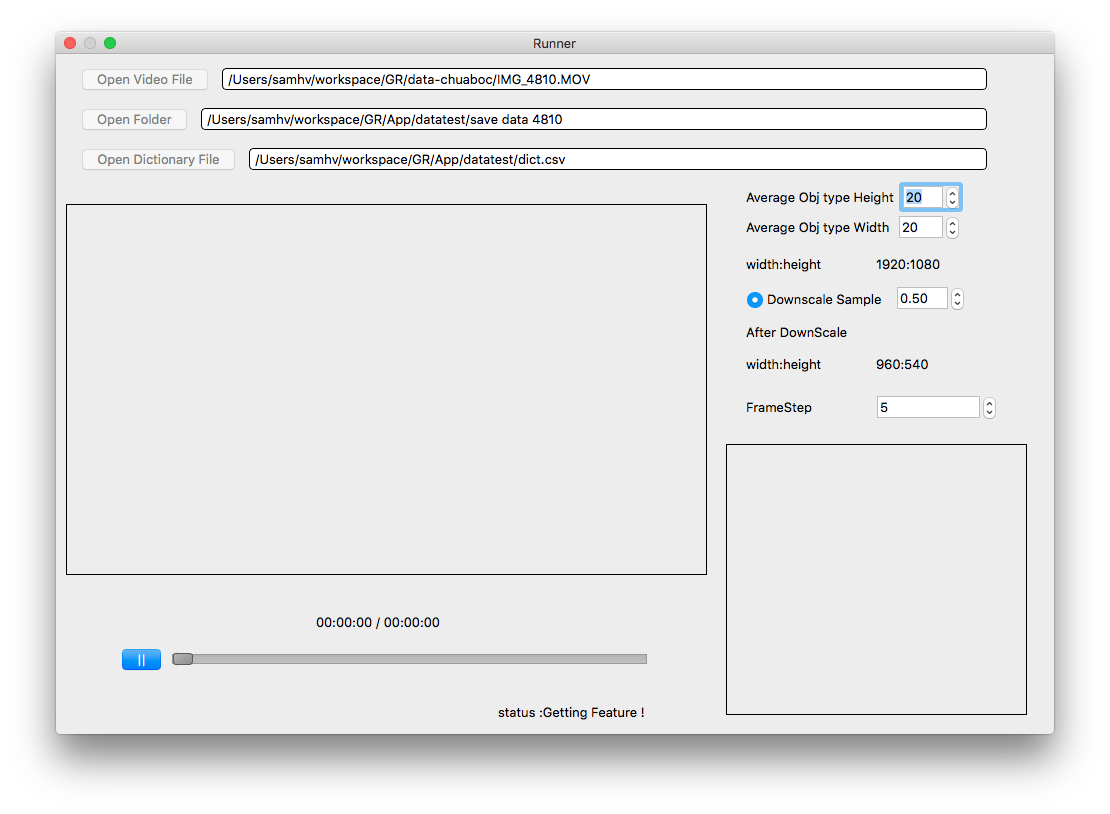
\includegraphics[width=\textwidth]{Chapters/Fig/Runner}
      \caption{The Run Dialog}
      \label{fig:Runner}
  \end{figure}
\end{center}
Fig \ref{fig:Runner} shows the run dialog. The client needs to click on Open Video File button for choosing the video file that client needs to estimate the number of object for each object types has been defined on setting tab of marker dialog. Client clicks Open Folder button to choose the folder that contains results from the marker, trainer dialog. Client needs to click open dictionary file button to set the dictionary file for the creating features state in the estimation process. \textbf{Average size ob types height: } that set the value of dense SIFT height setting. \textbf{Average size ob types width: } that set the value of dense SIFT width setting. \textbf{Downscale sample: } is the ratio of sample with frame after downscale if it checks. \textbf{Frame set: } is the number of the frame between 2 continuous samples. Click $>$ for start estimation number of object for each object types. 
\begin{center}
  \begin{figure}[H]
    \includegraphics[width=\textwidth]{Chapters/Fig/Running}
    \caption{The Running Screen of Runner Dialog}
    \label{fig:running}
\end{figure}
\end{center}

\section{Results}
\subsection{Estimation Results}
  \begin{table}[H]
    \begin{center}
      \begin{tabular}{ | c | c | c |} 
        \hline
        & \textbf{Motor} & \textbf{Car} \\
        \hline
        \textbf{Gauss Ksize} &  48 &  72 \\
        \hline
        \textbf{Gauss Sigma} &  8 &  12 \\
        \hline
        \textbf{Number of Images} &  15 &  15 \\
        \hline
        \textbf{Number of Training Train} &  6 &  6 \\
        \hline
        \textbf{Number of Features} &  256 &  256 \\
        \hline
        \textbf{Max Iterations} &  50 &  50 \\
        \hline
        \textbf{Number of BinX for Sift feature} &  4 &  4 \\
        \hline
        \textbf{Number of BinX for Sift feature} &  4 &  4 \\
        \hline
        \textbf{Number of BinT for Sift feature} &  8 &  8 \\
        \hline
        \textbf{Bin Size X for Sift feature} &  12 &  18 \\
        \hline
        \textbf{Bin Size Y for Sift feature} &  12 &  18 \\
        \hline
         \textbf{Average True Count} & 15.723175 & 2.045831 \\
         \hline
         \textbf{Avg Error} & 2.206202 & 0.468913 \\
         \hline
         \textbf{Avg Error / True Count } & 0.144842 & 0.229204 \\
       \hline
      \end{tabular}
    \end{center}
    \caption{Estimation Result From models Trained Separately}\label{tab:data}
  \end{table}

  \begin{table}[H]
    \begin{center}
      \begin{tabular}{ | c | c | c |} 
        \hline
        \textbf{Image} & \textbf{True Count} & \textbf{Model Count}  \\
        \hline
        7 &  27.3 &  27.6 \\
        \hline
        8 &  24.7 &  29.6 \\
        \hline
        9 &  18.3 &  19.07 \\
        \hline
        10 &  5.4 &  8.2 \\
        \hline
        11 &  11.3 &  14.3 \\
        \hline
        12 &  10.1 &  14.7 \\
        \hline
        13 &  14.3 &  16.1 \\
        \hline
        14 &  14.6 &  15.09 \\
        \hline
        15 &  15.13 &  16.3 \\
       \hline
      \end{tabular}
    \end{center}
    \caption{Estimation Result in Details for Motor}\label{tab:data-motor}
  \end{table}

  \begin{table}[H]
    \begin{center}
      \begin{tabular}{ | c | c | c |} 
        \hline
        \textbf{Image} & \textbf{True Count} & \textbf{Model Count}  \\
        \hline
        7 &  4.11&  4.61 \\
        \hline
        8 &  4.35 &  5.10 \\
        \hline
        9 &  4.26 &  3.3 \\
        \hline
        10 &  2.00 &  1.77 \\
        \hline
        11 &  0.00 &  0.52 \\
        \hline
        12 &  0.09 &  0.52 \\
        \hline
        13 &  1.00 &  1.01 \\
        \hline
        14 &  1.12 &  1.48 \\
        \hline
        15 &  1.46 &  2.09 \\
       \hline
      \end{tabular}
    \end{center}
    \caption{Estimation Result in Details for Car}\label{tab:data-car}
  \end{table}
  % \textit{Note: the images 7 to 15 are show in appendice \ref{app:01}.}

  \begin{center}
    \begin{figure}[H]
        \centering
      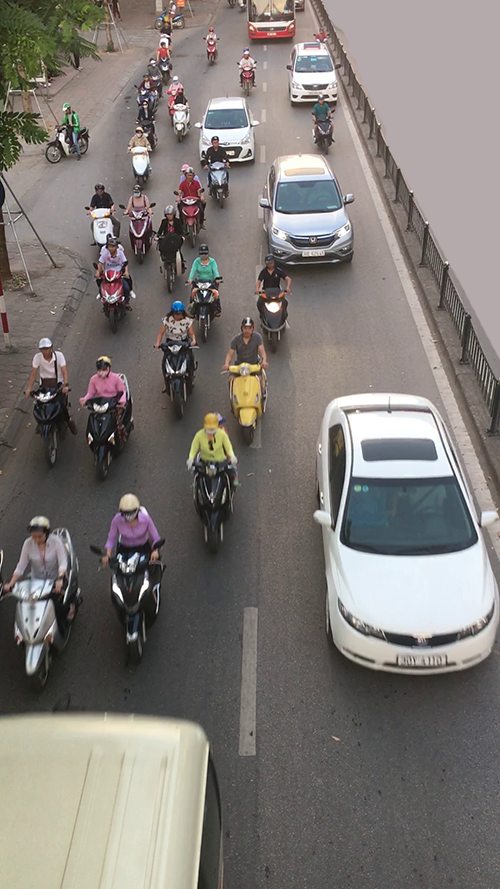
\includegraphics[width=0.5\textwidth]{Chapters/Fig/07}
      \caption{Image 7}
      \label{fig:img07}
  \end{figure}
\end{center}

\begin{center}
    \begin{figure}[H]
        \centering
      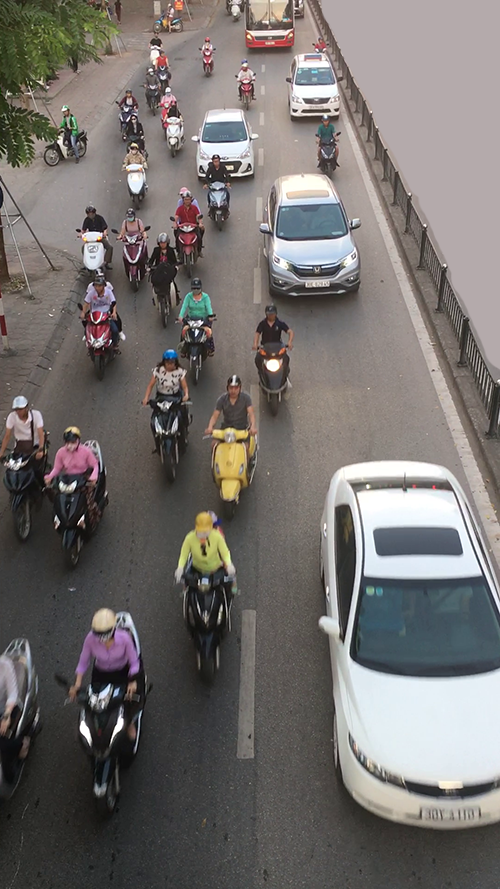
\includegraphics[width=0.7\textwidth]{Chapters/Fig/08}
      \caption{Image 8}
      \label{fig:img08}
  \end{figure}
\end{center}

\begin{center}
    \begin{figure}[H]
        \centering
      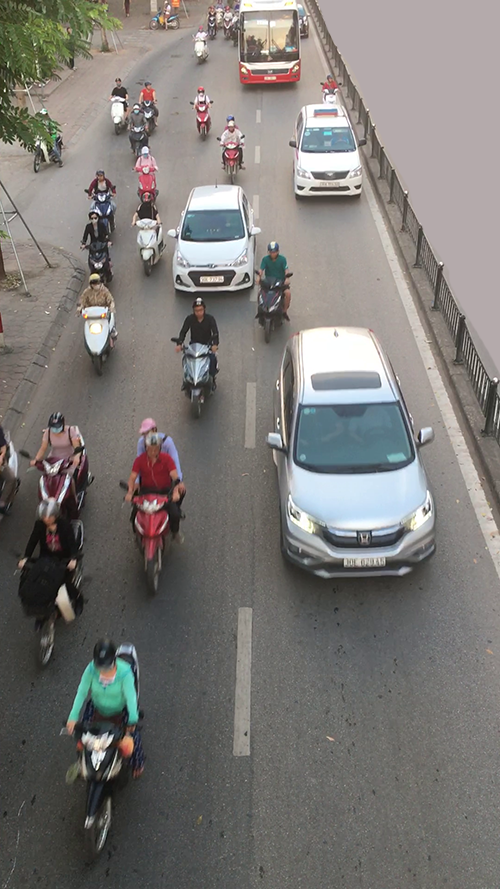
\includegraphics[width=0.7\textwidth]{Chapters/Fig/09}
      \caption{Image 1}
      \label{fig:img09}
  \end{figure}
\end{center}

The result form table \ref{tab:data} is the result of the learning function that Implement from learning method proposed by
Lempitsky V, Zisserman A \cite{Lempitsky:Zisserman:Destimate}. The result is good with average ratio error over true count approximate 0.14 for motors and 0.22 for cars. The problems cause the number of object estimate still have error are:
  \begin{enumerate}
    \item Training set did not make enough.
    \item Number of the object in training set did not enough.
    \item Images of training set has noise such as two lanes with opposite direction, tree, fence in between 2 lanes.
    \item The perspective of images.
  \end{enumerate}
  The solutions for problems above are: 
  \begin{enumerate}
    \item Add more images to training set did not enough.
    \item Capture the images have more objects.
    \item Add region of interest in training state and estimation state. 
    \item Solve the perspective of images or choose the angle that perspective does not affect too much. 
  \end{enumerate}
  The application has solved one of the problems above by helping the client create images for training set with Marker.\\
  
%   \begin{center}
%     \begin{figure}[H]
%       \centering
%       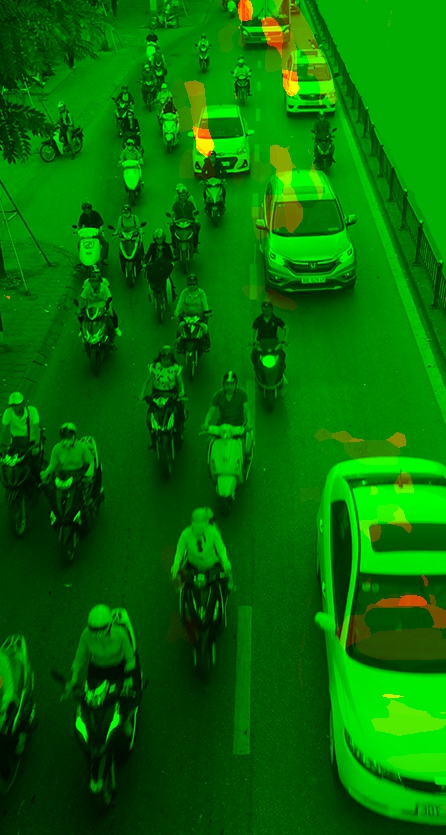
\includegraphics[height=0.5\textheight]{Chapters/Fig/car}
%       \caption{Example of Estimated Density for Cars}
%       \label{fig:ed-car}
%     \end{figure}
%   \begin{figure}[H]
%     \centering
%     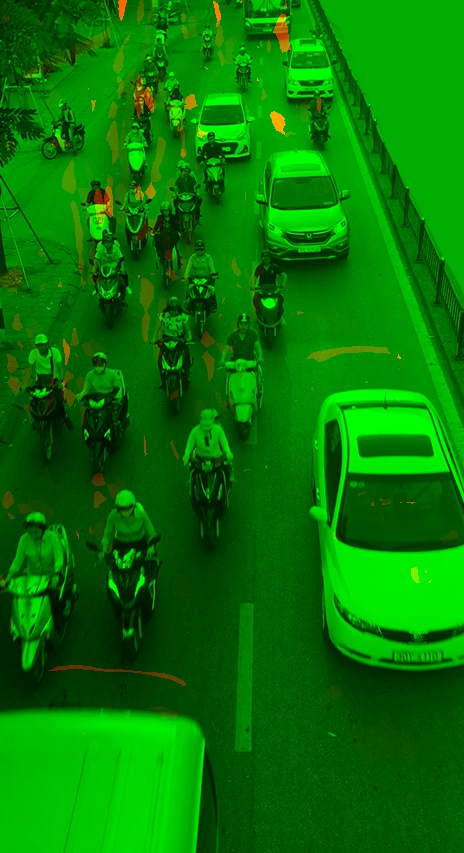
\includegraphics[height=0.5\textheight]{Chapters/Fig/motor}
%     \caption{Example of Estimated Density for Motors}
%     \label{fig:ed-motor}
%   \end{figure}
% \end{center}

%   The figure \ref{fig:ed-car} has the density almost located cars corretly. But the density of motor not located corretly. The reason is 2 object types has been set the gauss shaped is circle not the elipse. In the case of cars, the raito of height over width approximate is 2. Raito of height over width for motors approximate is 4. So that the cars located corretly than motors. In the application has been add the feature that allow client set the height and width. 


  \subsection{Application Results}

  The application has sucessful implement the feature: 
  \begin{enumerate}
    \item Marker: support client creates the training set for multi-kinds for object.  
    \item Trainer: support client train model for multi-kinds with training set from Marker. It has been integrated learning method proposed by Lempitsky V, Zisserman A \cite{Lempitsky:Zisserman:Destimate} for training state.
    \item Runner: support client estimate number of object for each type of object with models trained by Train.
  \end{enumerate}
  The application has been satisfied with the features, which has been propose in the early of this chapter. The result of the application on figure \ref{fig:running} not good because the client in marker did not create enough training images or did not mark all object of object types.

  \subsection{Time Measure For Estimation State In Application}
  \begin{table}[H]
    \begin{center}
      \begin{tabular}{ | c | c | c |} 
        \hline
        \textbf{Time} & \textbf{Width:Height}  \\
        \hline
        \textbf{4.3 second} &  576:324 \\
        \hline
        \textbf{1.8 second} &  384:216  \\
        \hline
      \end{tabular}
    \end{center}
    \caption{Time Measure for Estimation State}\label{tab:timeconsier}
  \end{table}

  From table \ref{tab:timeconsier}, it can be seen that the resolution 576:324 has 4 second to estimate and 384:216 is 1 second so that the time is not fast but still acceptable for the job counting multi-kinds of different objects in the dense crowd. Time for estimation number of object in each object type can be reduced by improving assign SIFT feature to the word in dictionary process. 